% Packages
% sudo tlmgr install silence appendixnumberbeamer fira fontaxes mwe noto csquotes babel helvet
%--- Preamble ---------------------------------------------------------%
% Load LaTeX packages
\documentclass[aspectratio=169]{beamer}                    % supports floating text in any location
\usetheme[darkmode]{pureminimalistic}
%\usetheme[lightmode]{pureminimalistic}
\graphicspath{{logos/}}
\usepackage{graphicx}

\usepackage[utf8]{inputenc}
\usepackage{csquotes,xpatch}% recommended
%\usepackage[english]{babel}
%\usepackage[american]{babel}
\usepackage[brazil]{babel}
\babelprovide[import, main]{portuguese}
\babelprovide[import]{english}
\usepackage{tikz}

% \renewcommand{\pageword}{}
\renewcommand{\logotitle}{\includegraphics%
   [width=.25\linewidth]{Images/logo.png}}
\renewcommand{\logoheader}{\includegraphics%
   [width=.5\linewidth]{Galaxies.png}}
\renewcommand{\logofooter}{\includegraphics%
   [width=.15\linewidth]{Galaxies.png}}


 
% \renewcommand{\logoheader}{\vspace{1.5em}}

\usepackage[
%    natbib=true,
    backend=biber,
%    style=abnt,
%    style=authoryear-comp,
%    style=authoryear,
    style=ieee,
%    style=acm,
%    style=apalike,
%    style=siam,
%    style=ieeetr,
%    style=plain,
    doi=true,
    eprint=false,
    hyperref=true]
    {biblatex}
\addbibresource{demo_bib.bib}

%% this makes it possible to add backup slides, without counting them
\usepackage{appendixnumberbeamer}
\renewcommand{\appendixname}{\texorpdfstring{\translate{appendix}}{appendix}}

% logos

% footer page
\setbeamertemplate{footline}{HUBBLE CONSTANT DISCREPANCY  |  Team VOYAGER}

\renewcommand{\pageword}{Slide}

% Math Font Default (Fira is strange)
\renewcommand\mathfamilydefault{\rmdefault}



% if loaded after begin{document} a warning will appear: "pdfauthor already used"
\title{\LARGE{\underline{\textbf {HUBBLE CONSTANT DISCREPANCY}}}}
\author{\large{\textit{Team VOYAGER \\ (Astrophysics)}}}
\date{\today}

\setbeamertemplate{background}{%
    \tikz[overlay,remember picture]%
    \node[opacity=0.4]at (current page.center)%
    {\includegraphics[width=.55\linewidth]%
        {Galaxies.png}};}


\begin{document}


% has to be loaded outside of a frame to work!
\maketitle
    
% For longer table of contents, I find it cleaner to
% use no footline.
\begin{frame}{Acknowledgement}
We would like to thank Mr. Sujay Sreedhar and Ms. Nikhitha C , co-founders of SSERD for giving us this  opportunity.

We are grateful to Mr. Mahesh and Mr. Pavan Kumar for providing us guidance and support throughout the period of work.

We would like to thank our mentor Mr. Sundar and our coordinator Ms. Anisha for their valuable inputs.
\end{frame}
\begin{frame}{Team memebers}
     \centering \large {Bhuvaneshwari Kashi\\ Samarth Gujrati \\Sarvesh Kulkarni \\ Sanjana Bapna \\ Sharuk Aumi\\ Aishwarya Satyajith\\ Satvi Sanghani\\ Nithin Kishore \\ Priyam Gupta \\ Nachiket Jhala}
\end{frame}

\begin{frame}[plain, noframenumbering]{Outline}
    \tableofcontents
    \vfill
\end{frame}

\section{Problem Statement}
\begin{frame}[fragile]{Problem Statement}
   \large{ To compare different methods used to calculate Hubble's constant and analyse the discrepancy among them, also stating the probable reasons for the same.}
\end{frame}

\section{Introduction}
\begin{frame}{Introduction}
    \begin{columns}
    \column{0.5\textwidth}
    \begin{vfilleditems}
        \item 1929- observation of expansion of universe by Edwin Hubble
        \item Hubble’s law - Recessional velocity directly proportional to distance $V = H_0d$
        \item Hubble’s constant - describes the rate of expansion of universe
        \item Different methods were used 
        \item We have different values of H0
        \item Let's look at them
    \end{vfilleditems}
    \column{0.6\textwidth}
    \begin{figure}
        \centering
        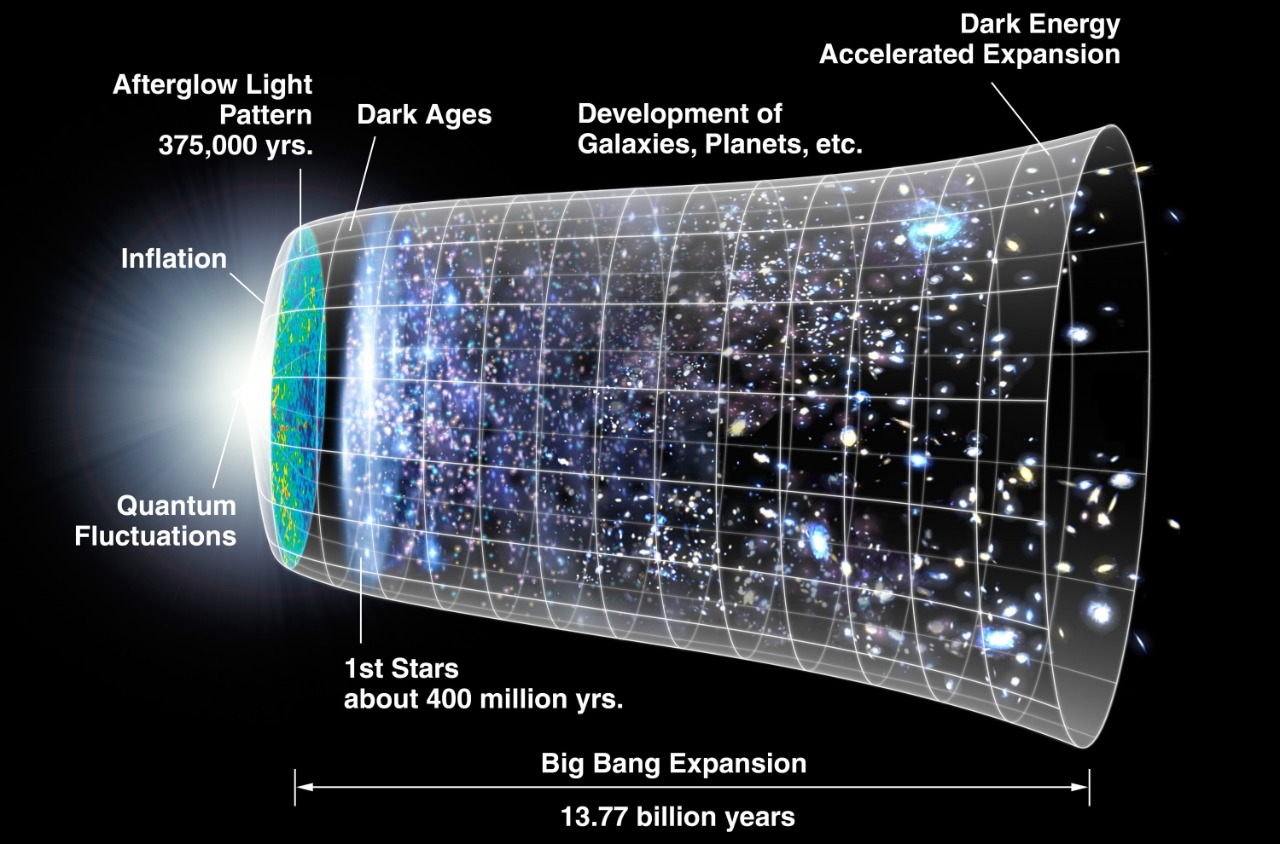
\includegraphics[width=8cm]{Images/WhatsApp Image 2021-06-04 at 13.07.12.jpeg}
        \caption{credit:NASA/WMAP Science Team}
        \label{fig:expansion}
    \end{figure}
    \end{columns}
\end{frame}


\section{Cepheid Variables}
\begin{frame}{Cosmic Distance Ladder}
\graphicspath{ {./Images/} }
    \begin{columns}
    \column{0.5\textwidth}
    %\begin{verbatim}
    %Use the provided \vfilleditems environment
    %to create nicely spaced bullet points.

    \begin{vfilleditems}
      \item Velocity can be calculated from redshifts: \par v $=$ cz, where c is the speed of light and z is the redshift.
      \item Calculating distance can be tricky.
      \item Hence Cosmic Distance Ladder method.
    \end{vfilleditems}
    
    \column{0.6\textwidth}
    \begin{figure}
        \centering
        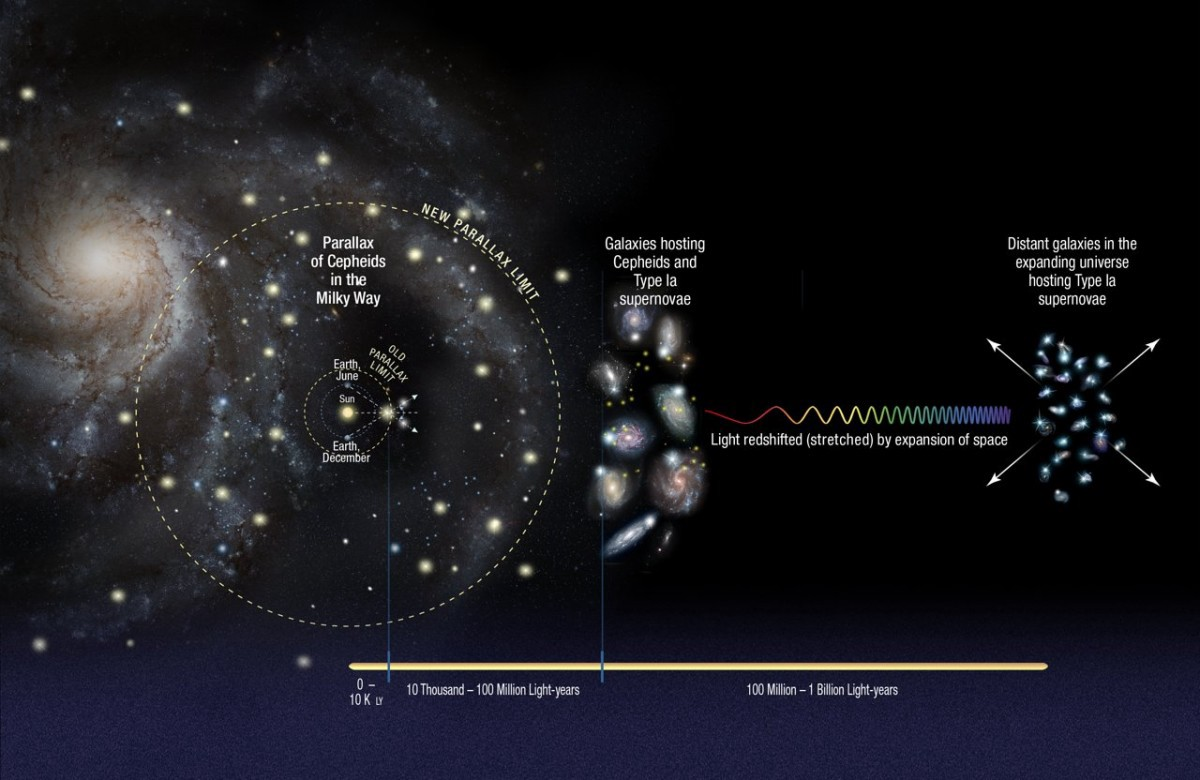
\includegraphics[width=8cm]{CDL1.jpg}
        \caption{The Cosmic Distance Ladder Method}
        \label{fig:CDL}
    \end{figure}
    \end{columns}
\end{frame}
\begin{frame}{Type 1 Cepheids}
\graphicspath{ {./Images/} }
    \begin{columns}
    \column{0.5\textwidth}
        
    \begin{vfilleditems}
        \item Standard Candles
        \item First Candidate---Type 1 Cepheids
        \item Luminosity directly proportional to Time Period
    \end{vfilleditems}
    \column{0.5\textwidth}
    \begin{figure}
       \centering
       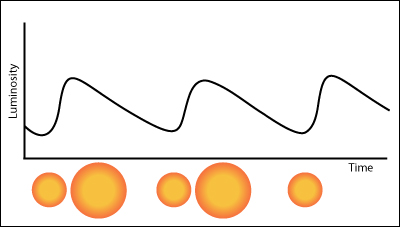
\includegraphics[width=6cm]{cepheid-variable time curve}
       \caption{Luminosity vs Time Period}
       \label{fig:my_label}
    \end{figure}
    \end{columns}
\end{frame}

\begin{frame}{Type 1 Cepheids}
\graphicspath{ {./Images/} }
    \begin{columns}
    \column{0.5\textwidth}
    
    \begin{vfilleditems}
        \item $M $=$ -2.78\log P-1.35$, where M is the absolute magnitude and P is time period
        \item $d$=$ 10^{(m-M+5)/5}$, where d is the distance and m is the apparent magnitude
        \item Multiple Cepheid in a galaxy, estimate the distance to the galaxy
    \end{vfilleditems}
    \column{0.5\textwidth}
    \begin{figure}
        \centering
        \includegraphics[scale=4]{Cepheid magnitude}
        \caption{Absolute magnitude vs Period}
        \label{fig:my_label}
    \end{figure}
    \end{columns}
\end{frame}


\section{Type Ia Supernova}
\begin{frame}{Type Ia Supernova}
    \begin{vfilleditems}
        \item Definition: Type of supernova that occurs in binary systems in which one of the stars orbiting the other one is a white dwarf. The other star can be anything from a giant star to an even smaller white dwarf
        \item Here, we analyse SNe Ia as standard candles in the near-infrared (NIR) in their peak J-band magnitudes 
        \item Reason: Fairly consistent peak luminosity because of fixed critical mass, which is also comparable to entire galaxies of moderate luminosity, and hence can be observed to distances of hundreds of Mpc
        \item Advantages: Lower intrinsic scatter than in the optical, reduced effects of dust
    \end{vfilleditems}
    
\end{frame}

\begin{frame}{Type Ia Supernova Data and Calculations}
    \begin{vfilleditems}
        \item Hubble-flow sample from SNe with NIR photometry was compiled from Vizier - Updated calibration of the CSP-I SNe Ia sample (Burns+, 2018)
        \item $z(hel) * 300000 = $Radial Velocity $(km/s)$
        \item Distance mod. muCV gives Distance (Mpc) through:
        $d = 10^{0.2(muCV+5)} * 10^{-6}$ $Mpc$
        \item On plotting the Radial Velocity vs Distance (Mpc) graph:
        
        Slope of the graph $= H_0 = 68.677$ $km/s.Mpc$
    \end{vfilleditems}
    
\end{frame}

\begin{frame}{Graph}
    \begin{figure}[htp]
        \centering
        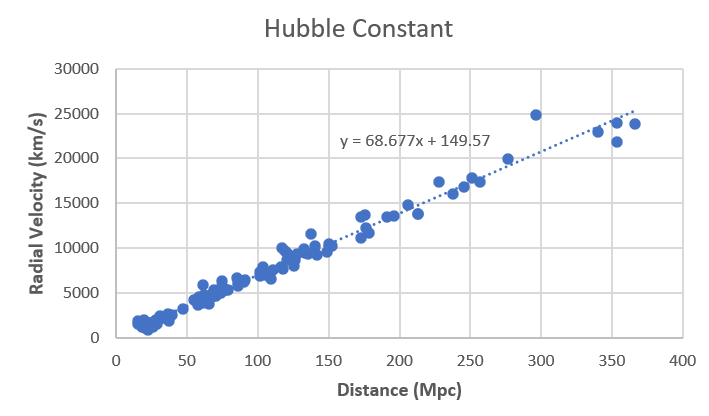
\includegraphics[width=10cm]{Images/Type Ia SN graph final.png}
        \caption{Hubble constant calculated from the data collected}
        \label{fig:Type Ia SN graph final}
    \end{figure}
\end{frame}

\begin{frame}{Errors in CDL}
    \begin{vfilleditems}
        \item Exact mechanism for the ignition of the explosion has not yet been theoretically or observationally established
        \item Theoretical astronomers long believed that the progenitor star for this type of supernova is a white dwarf, but there is no certainty
        \item Dependence of the period-luminosity relation on metallicity has not yet been accurately established
    \end{vfilleditems}
    
\end{frame}

\begin{frame}{Errors in CDL}
    \begin{vfilleditems}
        \item Reddening : Selective absorption and scattering of light by interstellar grains
        \item Peculiar Motion : Velocity due to gravitational effects of the other galaxies or clusters. $V_{total} = H_{o}*D + V_{pec}$
        \item Objects misidentified as cepheids while taking the observations
        

    \end{vfilleditems}
    
\end{frame}
\section{Gravitational Lensing}
\begin{frame}{Gravitational Lensing}
    \begin{vfilleditems}
        \item Gravitational lensing :As the light emitted by distant galaxies passes by massive objects in the universe, the gravitational pull from these objects can distort or bend the light. 
        \item The light travel time from source to the observer depends on both their path length and gravitational potential.
        \item Time delay: $t(\theta,\beta) = D _ \triangle t / c [((\theta -\beta)^2 /2)-\psi(\theta)] $
        \item Time delay distance : $D _ \triangle t = (1 + z_d) D_dD_s/D_d_s$
        \item The value of H0 from flat $\wedge$ CDM cosmology where constraints are used from strong lenses is found to be$73.3_-_1_._8^+^1^.^7 km s^-^1Mpc^-^1$,a 2.4\% precision measurement.
    \end{vfilleditems}
\end{frame}

\begin{frame}{Graph}
    \begin{figure}[htp]
        \centering
        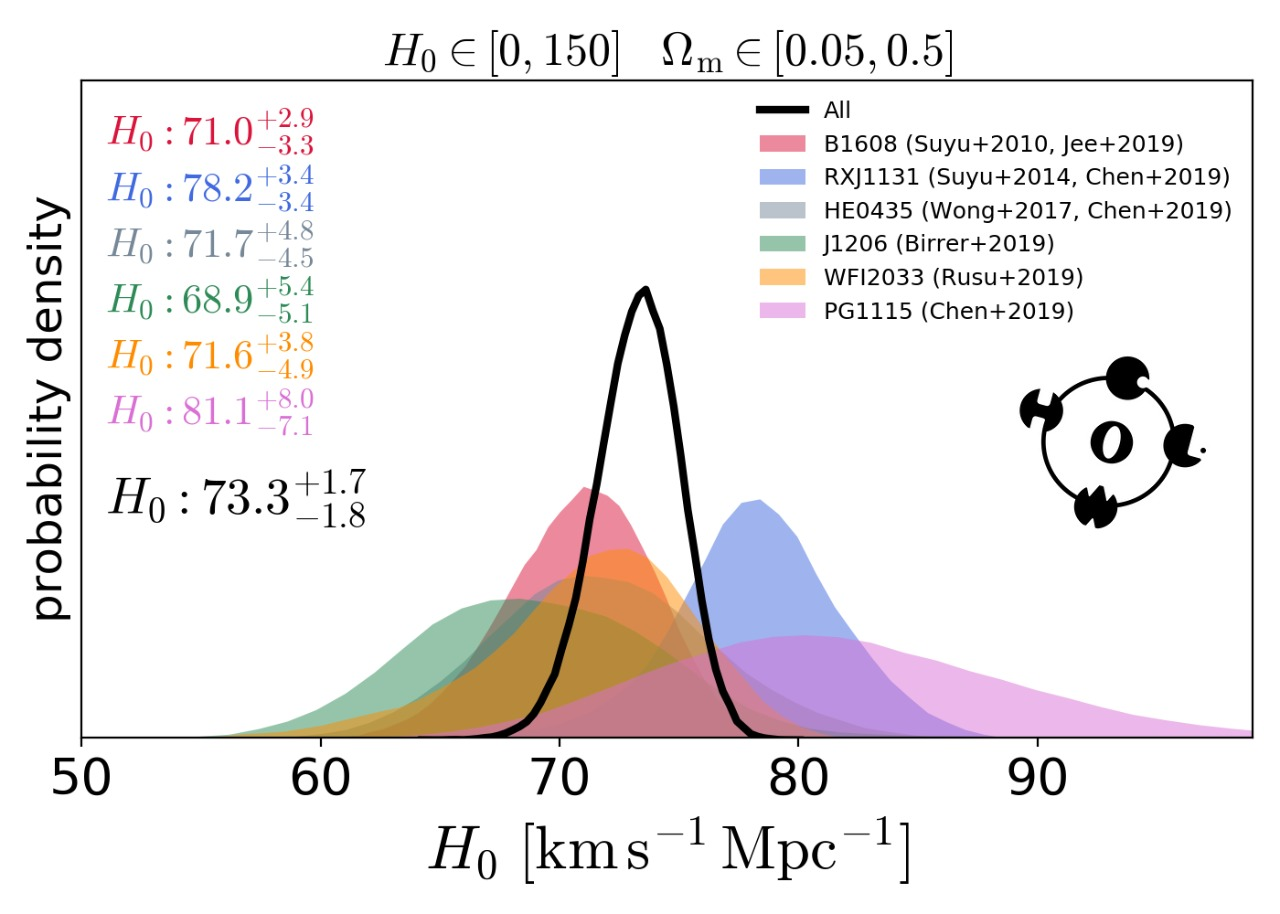
\includegraphics[width=9cm]{Images/Lensing_graph.png}
        \caption{Resource : H0L\emph{i}COW XIII: A 2.4\% measurement of H_0}
        \label{fig:Lensing_graph}
    \end{figure}
\end{frame}



\section{CMB Model and H0}
\begin{frame}{CMB Model and H0}
    \begin{vfilleditems}
        \item The cosmic microwave background, in Big Bang cosmology, is electromagnetic radiation which is a remnant from an early stage of the universe.
        \item To get the Hubble's constant we use the planck satellite analysis of CMB from which we first figure out what starting cosmological parameters could give the power spectrum observed by plank. Parameters like the starting combination of both dark and light matter, radiation and the initial expansion rate.
        Then we calculate how a universe with these parameters should evolve to the present day.
        \item The value of $H_0$ from this method has higher precision than all the other methods being $67.6 \pm 0.3$ $km s^-1 Mpc^-1$ which is only about $1/2\%$
    \end{vfilleditems}
\end{frame}

\section{Discrepancy in the value of H0}
\begin{frame}{Discrepancy in the value of H0}
    \begin{vfilleditems}
        
        \item Type Ia Supernovae: $68.677$ $km s^-1 Mpc^-1$
        \item Gravitational Lensing:$73.3_-_1_._8^+^1^.^7 km s^-^1Mpc^-^1$
        \item Cosmic Microwave Background: $67.6 \pm 0.3$ $km s^-1 Mpc^-1$
    \end{vfilleditems}
\end{frame}

\section{Possible reasons for discrepancy}
\begin{frame}{Possible reasons for discrepancy }
    \large{Reasons that might cause discrepancy with CMB model include:}
    \begin{vfilleditems}
        \item Dark matter behaves differently
        \item Dark energy isn't constant
        \item New fast moving particles
    \end{vfilleditems}\\[0.5cm]
\end{frame}

\begin{frame}{Possible reasons for discrepancy}
    \large {Reasons that might cause discrepancy with Gravitational lensing model include:}
    \begin{vfilleditems}
        \item Ripples and warps in space-time.
        \iem Kilonova formed by black hole - neutron-star merger might emit dark radiation. 
        \item Redshift calculation for time delay.
    \end{vfilleditems}\\[0.4cm]
    \large {Reasons that might cause discrepancy with CDL model include:}\\
    \begin{vfilleditems}
        \item Compounding errors in distance ladder.
    \end{vfilleditems}
\end{frame}

\section{Conclusion}
\begin{frame}{Conclusion}
    \begin{vfilleditems}
        In this project, we have compared and analyzed the methods of finding the Hubble constant by cosmic distance ladder, cosmic microwave background and gravitational lensing. We then explored the possible reasons for the discrepancies.  
    \end{vfilleditems}


\end{frame}

\begin{frame}{}
    \begin{figure}[htp]
        \centering
        
\includegraphics[width=12cm]{Images/slide_34.jpg}
    \end{figure}
\end{frame}

\end{document}
